\documentclass[french]{article}
\usepackage{aeguill,aecompl,babel,tikz,geometry}
\usetikzlibrary{arrows}
\usepackage[T1]{fontenc}
\usepackage[utf8]{inputenc}
\pagestyle{empty}
\geometry{
paperwidth=18cm,
paperheight = 8cm,
left=0pt,
right=0pt,
top=2pt,
bottom=0pt
}
\tikzset{%
cat/.style={right=2cm,anchor=west,align=left},
subcat/.style={below=1cm,anchor=north west,draw=none,font=\em,align=left}
}
\newcommand{\cate}{%
\quad\footnotesize%
\textendash\  Montant%
}
\newcommand{\opera}{%
\quad\parbox[t]{2.9cm}{%
\tiny
\textendash\ Montant\\
\textendash\ Marge\\
\textendash\ Date de mise en considération\\
\textendash\ Date de fin de considération\\
\textendash\ Période\\
\textendash\ ?`Automatique?\\
}
}
\pgfdeclarelayer{background}
\pgfsetlayers{background,main}
\begin{document}
\centering
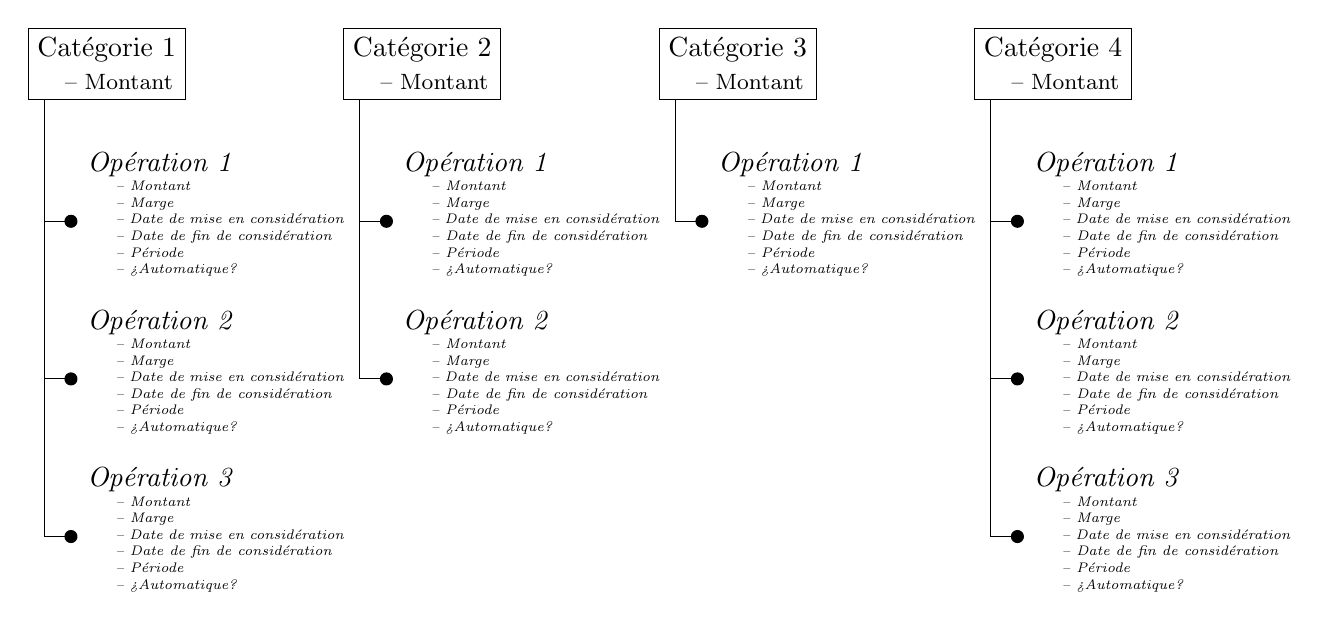
\begin{tikzpicture}[every node/.append style={draw,fill=white},
                    every path/.append style={-*}]
\node[align=left] (cat10) at (0,0) {Catégorie 1\\\cate};
\pgfmathparse{int(rnd*3 + 1)}\let\nsub\pgfmathresult
\foreach \subcat in {1,...,\nsub}
{
  \pgfmathparse{int(\subcat - 1)}\let\subcatbef\pgfmathresult
  \node[subcat] (cat1\subcat) at ([xshift=18pt]cat10.west |- cat1\subcatbef) {Opération \subcat\\[-5pt]\opera};
\begin{pgfonlayer}{background}
  \draw ([xshift=6pt]cat10.west |- cat1\subcatbef) |- (cat1\subcat);
\end{pgfonlayer}
}
\foreach \category in {2,...,4}
{
  \pgfmathparse{int(\category - 1)}\let\catbef\pgfmathresult
  \node[cat] (cat\category0) at (cat\catbef0.east) {Catégorie \category\\\cate};
  \pgfmathparse{int(rnd*3+1})\let\nsub\pgfmathresult
  \foreach \subcat in {1,...,\nsub}
  {
    \pgfmathparse{int(\subcat - 1)}\let\subcatbef\pgfmathresult
    \node[subcat] (cat\category\subcat) at ([xshift=18pt]cat\category0.west |- cat\category\subcatbef) {Opération \subcat\\[-5pt]\opera};
\begin{pgfonlayer}{background}
    \draw ([xshift=6pt]cat\category0.west |- cat\category\subcatbef) |- (cat\category\subcat);
\end{pgfonlayer}
  }
}

\end{tikzpicture}
\end{document}
